% -----------------------------------------------------------------------------
\section{Imported UML Classes}
% -----------------------------------------------------------------------------

PAML builds on the Unified Modeling Language (UML) version 2.5.1~\citep{uml251} to describe the organization of actions in a protocol.
In order to make this document more self-contained, this section describes the classes from UML that have been imported into PAML.
Rach such class has also been adapted to be an SBOL subclass, assigned to either \sbol{Identified} or \sbol{TopLevel}, in order to be able to be used with SBOL closure assumptions in an RDF environment.

\subsection{uml:ValueSpecification}
\label{sec:uml:ValueSpecification}

\begin{figure}[ht]
\begin{center}
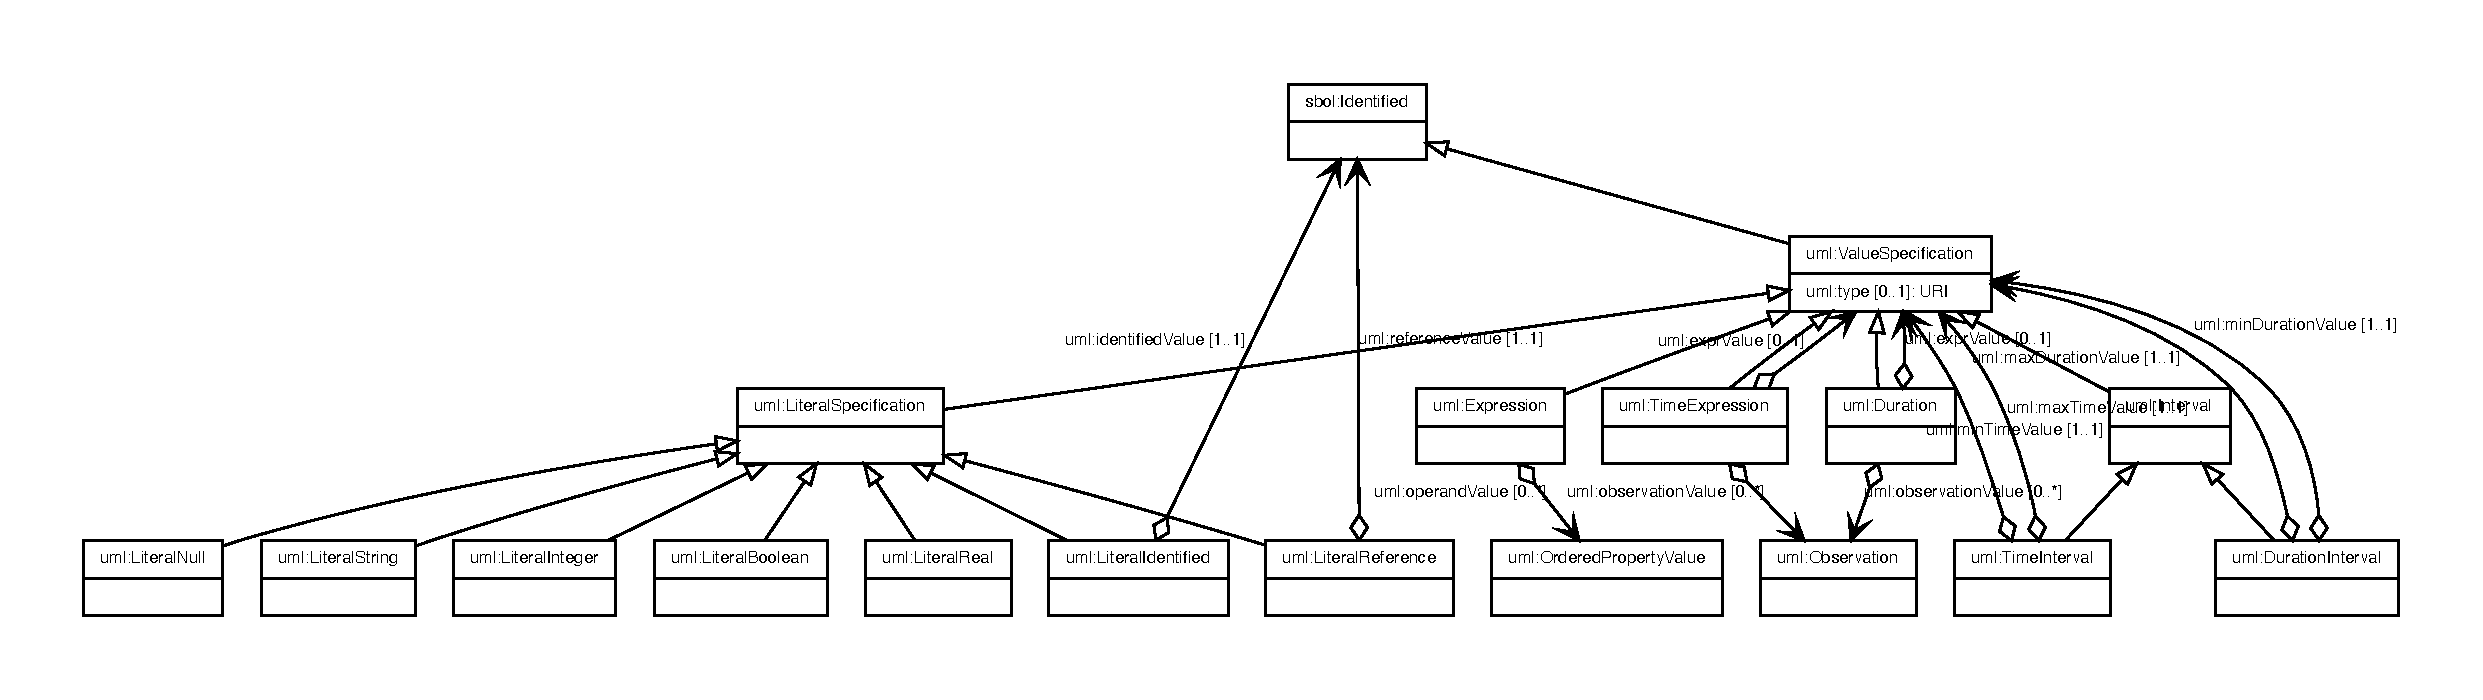
\includegraphics[scale=0.6]{uml_classes/ValueSpecification_abstraction_hierarchy.pdf}
\caption[]{Diagram of the XXX class and its associated properties}
\label{uml:ValueSpecification}
\end{center}
\end{figure}

%uml_classes/ValueSpecification_abstraction_hierarchy.pdf
%uml_classes/LiteralBoolean_abstraction_hierarchy.pdf
%uml_classes/LiteralInteger_abstraction_hierarchy.pdf
%uml_classes/LiteralNull_abstraction_hierarchy.pdf
%uml_classes/LiteralReal_abstraction_hierarchy.pdf
%uml_classes/LiteralSpecification_abstraction_hierarchy.pdf
%uml_classes/LiteralString_abstraction_hierarchy.pdf

\subsection{uml:Constraint}
\label{sec:uml:Constraint}

\begin{figure}[ht]
\begin{center}
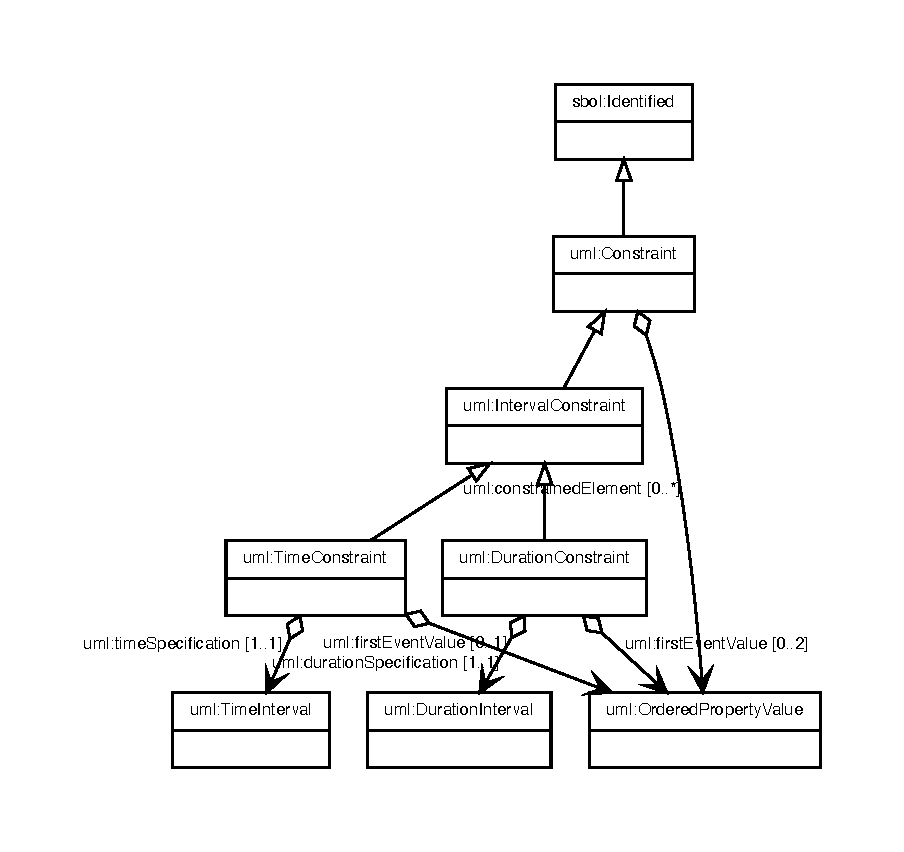
\includegraphics[scale=0.6]{uml_classes/Constraint_abstraction_hierarchy.pdf}
\caption[]{Diagram of the XXX class and its associated properties}
\label{uml:Constraint}
\end{center}
\end{figure}

%uml_classes/Constraint_abstraction_hierarchy.pdf

\subsection{uml:Parameter}
\label{sec:uml:Parameter}

\begin{figure}[ht]
\begin{center}
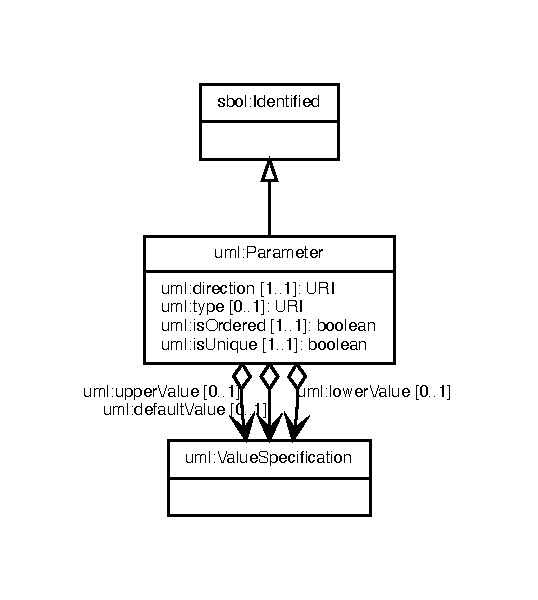
\includegraphics[scale=0.6]{uml_classes/Parameter_abstraction_hierarchy.pdf}
\caption[]{Diagram of the XXX class and its associated properties}
\label{uml:Parameter}
\end{center}
\end{figure}

%uml_classes/Parameter_abstraction_hierarchy.pdf

\subsection{uml:Behavior}
\label{sec:uml:Behavior}

\begin{figure}[ht]
\begin{center}
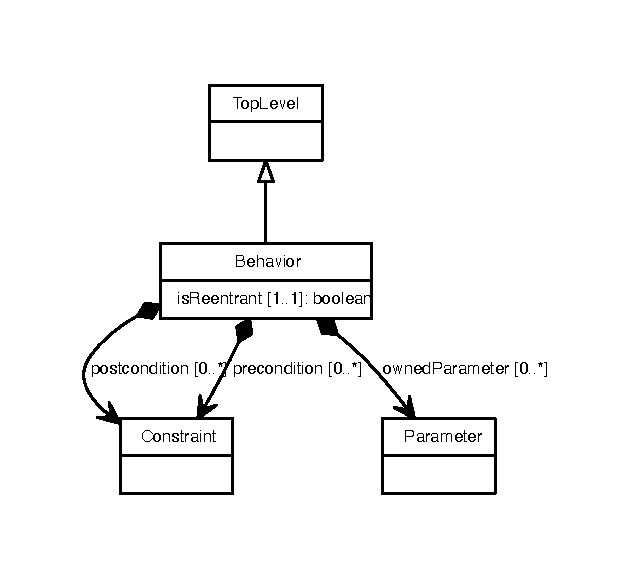
\includegraphics[scale=0.6]{uml_classes/Behavior_abstraction_hierarchy.pdf}
\caption[]{Diagram of the XXX class and its associated properties}
\label{uml:Behavior}
\end{center}
\end{figure}

%uml_classes/Behavior_abstraction_hierarchy.pdf
%uml_classes/Activity_abstraction_hierarchy.pdf

\subsection{uml:ActivityNode}
\label{sec:uml:ActivityNode}

\begin{figure}[ht]
\begin{center}
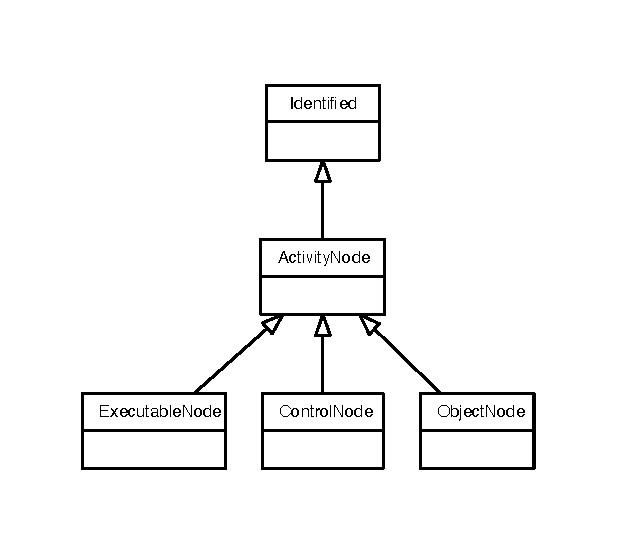
\includegraphics[scale=0.6]{uml_classes/ActivityNode_abstraction_hierarchy.pdf}
\caption[]{Diagram of the XXX class and its associated properties}
\label{uml:ActivityNode}
\end{center}
\end{figure}

%uml_classes/ActivityNode_abstraction_hierarchy.pdf
%uml_classes/ExecutableNode_abstraction_hierarchy.pdf
%uml_classes/Action_abstraction_hierarchy.pdf
%uml_classes/CallBehaviorAction_abstraction_hierarchy.pdf % includes CallAction, InvocationAction
%uml_classes/ControlNode_abstraction_hierarchy.pdf
%uml_classes/DecisionNode_abstraction_hierarchy.pdf
%uml_classes/FinalNode_abstraction_hierarchy.pdf
%uml_classes/FlowFinalNode_abstraction_hierarchy.pdf
%uml_classes/ForkNode_abstraction_hierarchy.pdf
%uml_classes/InitialNode_abstraction_hierarchy.pdf
%uml_classes/JoinNode_abstraction_hierarchy.pdf
%uml_classes/MergeNode_abstraction_hierarchy.pdf
%uml_classes/ObjectNode_abstraction_hierarchy.pdf
%uml_classes/ActivityParameterNode_abstraction_hierarchy.pdf
%uml_classes/Pin_abstraction_hierarchy.pdf
%uml_classes/InputPin_abstraction_hierarchy.pdf
%uml_classes/ValuePin_abstraction_hierarchy.pdf
%uml_classes/OutputPin_abstraction_hierarchy.pdf

\subsection{uml:ActivityEdge}
\label{sec:uml:ActivityEdge}

\begin{figure}[ht]
\begin{center}
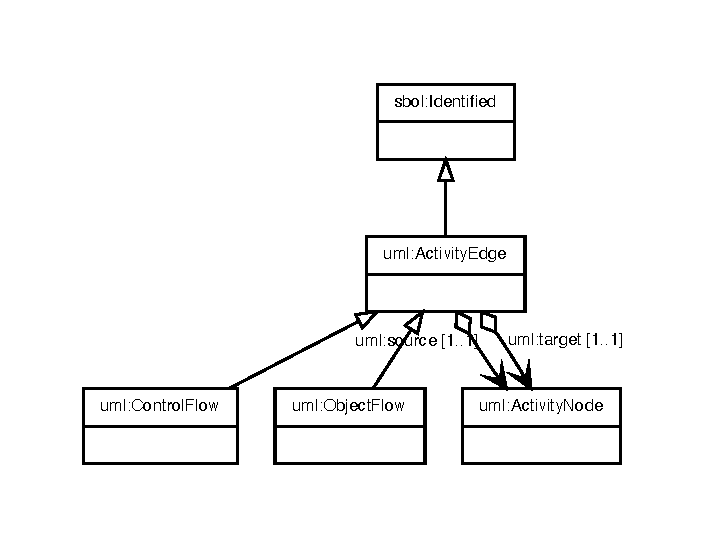
\includegraphics[scale=0.6]{uml_classes/ActivityEdge_abstraction_hierarchy.pdf}
\caption[]{Diagram of the XXX class and its associated properties}
\label{uml:ActivityEdge}
\end{center}
\end{figure}

%uml_classes/ActivityEdge_abstraction_hierarchy.pdf
%uml_classes/ControlFlow_abstraction_hierarchy.pdf
%uml_classes/ObjectFlow_abstraction_hierarchy.pdf

